
\documentclass[12pt]{article}
\usepackage{scrextend}
\usepackage[utf8]{inputenc}
\usepackage[polish]{babel}
\usepackage[T1]{fontenc}%polskie znaki
\usepackage[utf8]{inputenc}%polskie znaki
\usepackage{geometry}
\usepackage{float}
\usepackage{enumitem}
\usepackage{hyperref}
\usepackage{graphicx}
\usepackage{tabulary}
\usepackage{etoc}
\usepackage[normalem]{ulem} 
\usepackage{tikz}
\usepackage[bf]{caption}
\usepackage{amsmath}

\renewcommand{\baselinestretch}{1.5}

\usepackage{listings}
\usepackage{xcolor}
 
\definecolor{codegreen}{rgb}{0,0.6,0}
\definecolor{codegray}{rgb}{0.5,0.5,0.5}
\definecolor{codepurple}{rgb}{0.58,0,0.82}
\definecolor{backcolour}{rgb}{0.95,0.95,0.92}
 
\lstdefinestyle{mystyle}{
    backgroundcolor=\color{backcolour},   
    commentstyle=\color{codegreen},
    keywordstyle=\color{magenta},
    numberstyle=\tiny\color{codegray},
    stringstyle=\color{codepurple},
    basicstyle=\ttfamily\footnotesize,
    breakatwhitespace=false,         
    breaklines=true,                 
    captionpos=b,                    
    keepspaces=true,                 
    numbers=left,                    
    numbersep=5pt,                  
    showspaces=false,                
    showstringspaces=false,
    showtabs=false,                  
    tabsize=2
}
\renewcommand{\lstlistlistingname}{Spis listingów}\lstset{style=mystyle}

\graphicspath{ {img/} }
\newgeometry{lmargin=2.0cm, rmargin=2.0cm, tmargin=2.0cm, bmargin=2.0cm}
\clubpenalty=9996
\widowpenalty=9999
\brokenpenalty=4991
\predisplaypenalty=10000
\postdisplaypenalty=1549
\displaywidowpenalty=1602

\title{ 
    \vspace*{50mm}
    \textsc{
        \textbf{Rozpoznawanie i przetwarzanie obrazów}\\
        \large Sprawozdanie 
    }
} 
\author{
Damian Koper,  241292\\
Mateusz Gurski, 242089
}

\date{\today}

\begin{document}

\maketitle

\newpage
\setcounter{tocdepth}{2}
\localtableofcontents
\listoffigures 
\lstlistoflistings
\vfill
Kod i wersja wykonywalna programu: \url{https://github.com/damiankoper/ripo}
\newpage

\section{Uzyskane efekty}


%%%%%%%%%%%%%%%%
\begin{enumerate}
    
\item Przygotowane zostały wszystkie podstawowe peryferia. 

\begin{figure}[H]
    \centering
    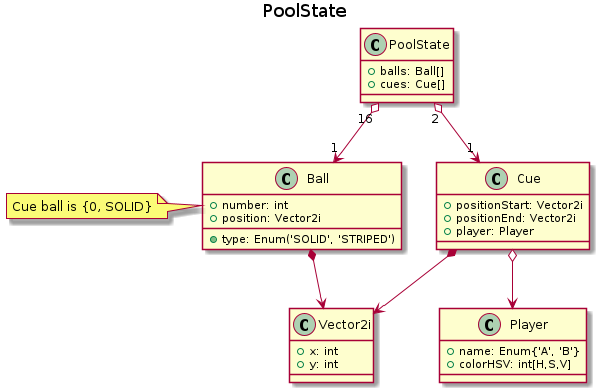
\includegraphics[width=10cm]{./diagrams/out/pull_state_cd.png}
    \caption{Struktura PoolState, przechowująca aktualny stan stołu}
    \label{}
\end{figure}

\begin{figure}[H]
    \centering
    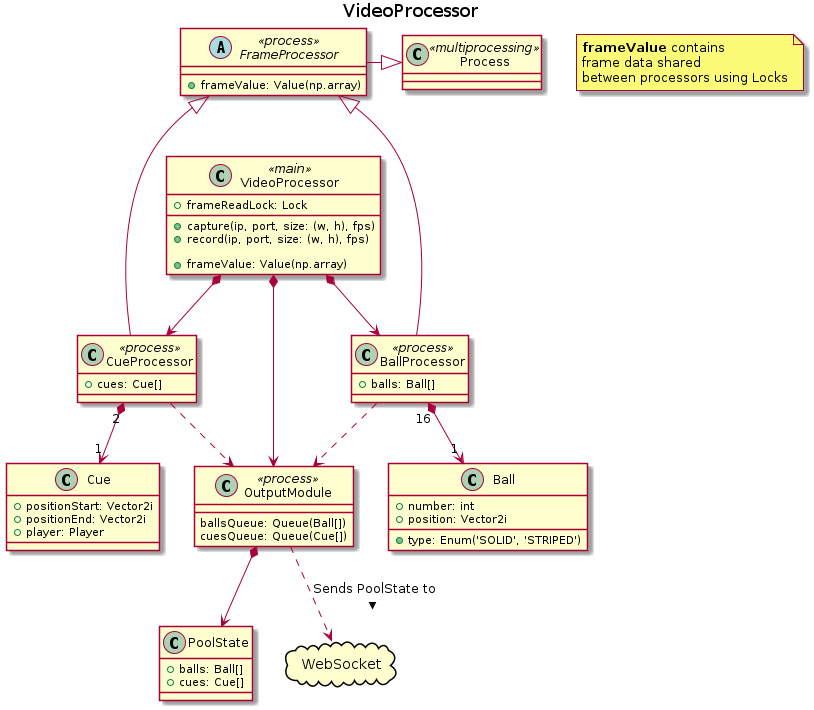
\includegraphics[width=14cm]{./diagrams/out/video_processor_cd.png}
    \caption{Struktura programu}
    \label{}
\end{figure}

\item Przygotowana została część wizualizacyjna, wyświetlająca aktualny stan stołu.

\begin{figure}[H]
    \centering
    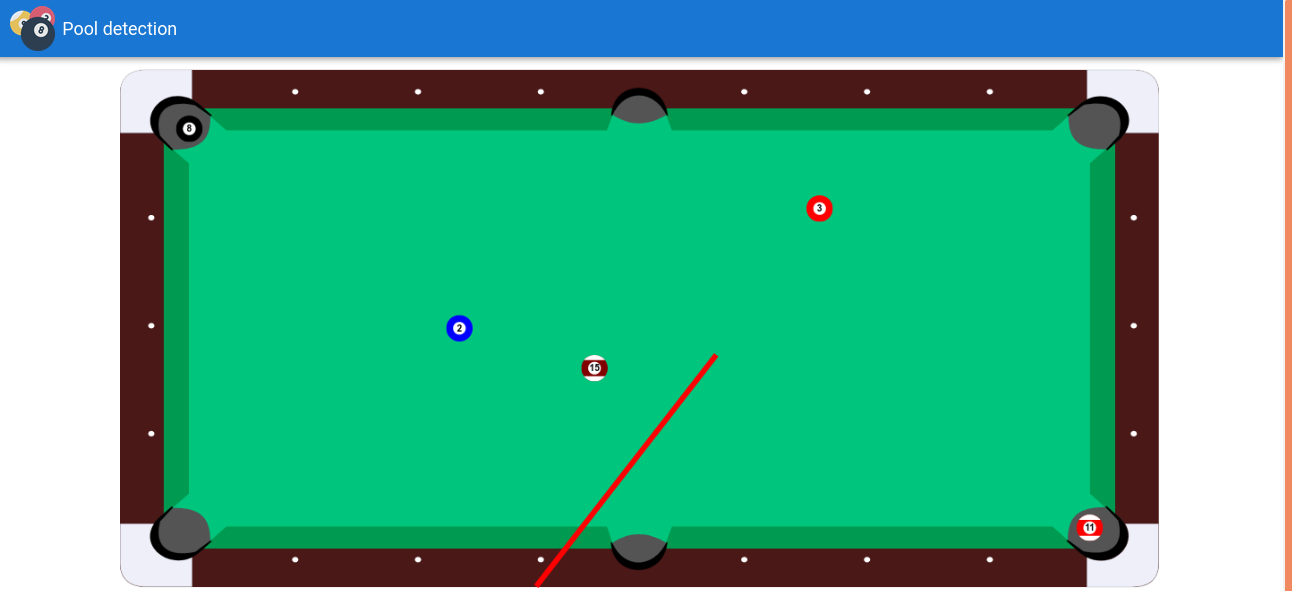
\includegraphics[width=10cm]{./diagrams/out/poolvd.png}
    \caption{Pool VD}
    \label{}
\end{figure}

\item Udało się zapewnić komunikację pomiędzy częścią backendową, odpowiadająca za rozpoznawanie i przetwarzanie oraz częścią frontendową, odpowiadająca za wizualizacje aktualnego stanu stołu.

\item W części backendowej wykorzystany został multiprocessing, utworzone zostały osobne procesy - VideoProcessor, BallProcessor, CueProcessor, OutputModule - pracujące równolegle i odpowiadające kolejno za odczyt kolejnych klatek, deteckję bil, 
detekcje kijów, zbieranie danych i komunikacje z częścią odpowiadającą za wizualizacje.

\item Rozdzielenie wejściowe poleceń. Wszystkie dane wejściowe podawane są podczas uruchamiania skryptu z odpowiednimi flagami. Oprócz tego utworzono 2 główne tryby uruchomieniowe: capture - tryb główny, odpowiadający za przechwytywanie i
przetwarzanie obrazu. Record - odpowiadający za nagrywanie przechwytywanego obrazu. 

\end{enumerate}


\vspace{2cm}



\end{document}